
\chapter{Approach}\label{chapter:approach}

In this chapter, the main approach of this thesis is presented. The chapter starts with an abstract description of the approach with the aim of providing a high-level overview of the underlying concepts. Then, exemplary use cases are described, and finally, a list of requirements and desirable quality attributes is given (\autoref{sec:requirements}) which forms the basis for the evaluation part in \autoref{chapter:discussion}. 

%
%
%
%
%
%
%
%
%
%

\section{Concept} \label{sec:concept}
The objective of this thesis is to explore a new method to handle the increased demand for computational power and data collection in mobile cyber-physical systems, and in particular, automotive systems. For this, an approach is presented that allows for the outsourcing of vehicular functions to the cloud.
A special requirement is the unreliable connectivity common to mobile systems. To deal with this, the solution must be able to perform the offloading in an instantaneous, fail-safe, and automated fashion. When cloud connectivity cannot be provided, the operation of the vehicle mustn't be affected in any way and the previous state must be reestablished as soon as connectivity is restored.

%the cohesion of the system must be preserved at all times. 

\subsection{Partitioning of Functionality}
At the core of the approach is the idea to split functionality into isolated units which may be deployed redundantly on both, the vehicle's on-board system, and on high-performance machines in remote data centers. For this, the system needs to facilitate the clean separation of functionality according to responsibilities. The \emph{service-oriented} architectural paradigm \cite{erl2008soa} is a proven method for achieving this \todo{citation: generell SOA}. Service-orientated architectures aim to divide functionality into isolated, loosely coupled modules, so-called \emph{services}. Each service provides an offering to users, or other services, by means of a clearly defined, preferably immutable and machine-readable interface. By guaranteeing that these interfaces rarely change, a formal \emph{service contract} is put in place which ensures the continuous interoperability between the services. Examples of a service offering may be the provisioning of some sort of data, or functionality (algorithms and business logic) that is executed on behalf of a service consumer. All services of the system are working together like cogs in a machine to achieve a common goal, \ie , the continuous operation of a vehicle. 


\subsection{Communication}
Traditionally, E/E-architectures build on the principle of message buses as means to connect the system's dispersed components (ECUs)\todo{citation?}. In bus systems, all components write data samples to, and read data samples from, a shared medium (the bus). Individual components typically have no knowledge of each other's existence---they only know the data they provide and push it on the bus, or read the data they are interested in from the bus. This paradigm leads to a loosely coupled system in which components have as few dependencies among each other as possible. Loose coupling, in turn, tremendously facilitates extensibility and scalability. A concept closely related to message buses is the publish-subscribe principle by which service providers (publishers) and service consumers (subscribers) communicate on the basis of topics. In effect, a publish-subscribe system behaves in accordance with a bus system in which the shared medium is logically segregated into domains (\ie\ topics). 

In line with the traditional bus-centered nature of E/E-systems, the presented approach builds on a bus-like publish-subscribe paradigm. The characteristic that makes the envisaged bus special is that it virtually extends into the cloud. To facilitate this, a \emph{network overlay} \cite{tarkoma2010overlay} mechanism is needed. With the help of a virtual overlay network laid on top of the substrate network, a globally dispersed \emph{service mesh} may be created wherein the boundaries of the physical network lose their effect. That way, location-transparent messaging between services is achieved: it does not matter whether a given service runs within the vehicle or within the cloud---the way they communicate remains the same.

%\paragraph{}

%The last question that remains is how services are connected. Since services may be duplicated and migrated between computing nodes, special emphasis needs to be put on location/relocation transparency and dynamic topology management. In the approach, the use of virtual overlay networks is suggested for this purpose. Especially challenging is the fact that the overlay must work on top of a substrate network made up of numerous globally dispersed nodes, of which some continuously change their location. As a result, the substrate network is exceptionally unreliable.


%An inherent challenge distinctive to the domain at hand is the highly unreliable and unpredictable communication channel to the cloud. Remotely deployed services are thus ephemeral in their nature. As a consequence, the topology of the service network is constantly changing. This requires the communication method between services to be entirely anonymous. \Ie , services shall not have references to other services as these may be unavailable momentarily. Management of references (addition of new references and invalidation of old ones) is highly ineffective and therefore should be avoided at all costs. A communication paradigm that facilitates this is the publish-subscribe paradigm. In a publish-subscribe system, services exchange information by means of topics. Services that provide data may push data on a given topic, and services that wish to receive that data may subscribe to that topic. Services do not know where a given data sample came from or which service will receive their data sample. Thus, communication is anonymous.

%\todo[inline]{

%Switch must be feasible at run-time

%transition must be fluent

%Communication shall be ubiquitous

%A major problem in automotive architectures is the management of data. As a result of the historically grown nature, whereby each ECU is highly specialized in a very narrow range of duties, there is no consistent model of data---each ECU has its own view on data which may very well differ from other ECU's view \cite{broy2006challenges}. It is therefore evident that data need to be put into the center of attention. Data-centricity is a communication style that follows this goal. provides common, consistent view on data. global shared data space.
%}

%The method of exposition is data-centric: instead of providing \emph{methods} that other services may invoke (RPC style), services offer \emph{data}. Any service interested in receiving a certain kind of data listens in on a topic on which such data is published. This approach greatly helps to decouple the system as services do not need to have references to one another. As a result, services may evolve without having to deal with interface interdependencies.


\subsection{Replication}
The approach aims to achieve superior computing performance by way of horizontal scaling. Thus, replication is key. 
%Thus, the system shall support the fast provisioning of services in the form of \emph{service instances}. 
The service-oriented approach alleviates replication tremendously, provided that certain design principles are applied. Hence, throughout the design and implementation of the envisaged system, several design goals need to be kept in mind. Firstly, services ought to be \textbf{stateless}. Statelessness facilitates replication as sharing state among many instances proves to be difficult. Consistency within a distributed system is hard to achieve and locking mechanisms may introduce bottlenecks.\todo{more on consistency models this in tanenbaum...} A common practice to remove the need for such mechanisms is to avoid state altogether. 

Furthermore, services should be \textbf{fine-grained}. A high-resolution granularity allows for detailed control over which services should be replicated. That way, computational bottlenecks can be more easily singled-out and eliminated. An added benefit of fine granularity is an increase in extensibility and faster software updates. However, trade-offs need to be considered. If services are too fine-grained, they need to communicate more which may slow down the system. Furthermore, too many services unnecessarily increase complexity.

Another design goal to keep in mind is \textbf{isolation}. Services should have limited knowledge of other services' location and the system's topology. Through this, loose coupling is further promoted. One aspect of isolation is self-containment. Services should be bundled together with all their dependencies as a single unit that may be deployed on any hardware platform. By packaging services in self-contained environments, they may be moved between different computing nodes. This property is the most important one to achieve cloud scalability. Commonly used tools to facilitate this are virtualization and containerization.

\subsection{Example}
\begin{figure}[htpb]
  \centering
  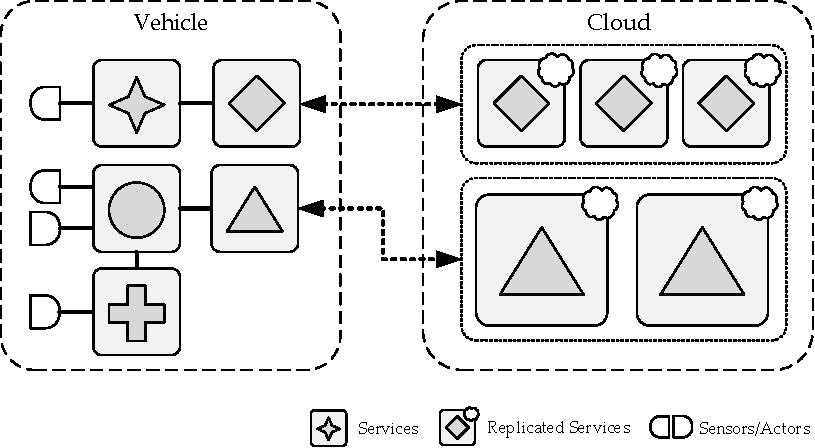
\includegraphics[width=0.9\textwidth]{figures/idea.pdf}
  \caption[Conceptual sketch of the approach]{Conceptual sketch of the approach}\label{fig:idea}
\end{figure}
\autoref{fig:idea} depicts a schematic example of the approach. The box on the left-hand side represents a vehicle. In the vehicle, several interconnected services are deployed. The figure omits any details regarding the actual computing infrastructure but only displays the general placement of services (either vehicle or cloud). In actuality, the the vehicular services run on distributed embedded devices spread over the vehicle's on-board system. Several of these services rely on sensor data and/or control actors (indicated by the small semicircles). On the right-hand side, the cloud is depicted, which, in actuality, is a collection of high-performance computing nodes. Vehicle and cloud are physically separated and connected via some sort of network, which the vehicle may access by means of cellular networking technology. On a logical level, vehicular- and cloud-based services communicate via topics that may, or may not, span between the two otherwise isolated systems. Note that some of the vehicle-intrinsic services are replicated in the cloud (\ding{117}, \ding{115}). Examples of such services could be functions for calculating trajectories, computer vision-based gaze detection, or machine learning applications. The duplication and varying size of the service boxes depicted in the image is indicative of horizontal and vertical scaling, respectively. It doesn't always make sense to replicate services in the cloud, \eg , because they are computationally inexpensive, or because they require access to sensors and actors which are inherently bound to the vehicle (\ding{70}, \ding{108}, \ding{58}). Those services have their firm place within the vehicle and are therefore referred to as \emph{fixed} services. Their counterpart, \ie , services that may run ubiquitously, are called \emph{volatile} services (\ding{117}, \ding{115}). A third kind of services are \emph{cloud-only} services, which are entirely optional and only serve to perform background tasks such as monitoring or persistence (\ding{86}, \ding{72}). Service \ding{72}, for example, would aggregate all data posted on Topic B and store it in a database. The discrepancy between fixed and volatile services emphasizes the need to split functionality into fine-grained services so that computational bottlenecks can be isolated and then eliminated. A good advice is to extract services connected to sensors and actors in minimal "access services" (\ding{70}, \ding{108}, \ding{58}) that do nothing but provide access to sensor data.
%
%
%
%
%
%
%
%
%
%
\subsection{Key Challenges} 
\label{sec:challenges}
In the previous sections, a conceptual approach was presented to connect a vehicle's on-board system to the cloud to facilitate computation offloading, data collection, and other use cases. To achieve this, the approach suggests to split functionality into fine-grained services that may be replicated and migrated smoothly between vehicle and cloud. Three key challenges can be identified which need to be addressed in order to realize the system:

\begin{enumerate}[(i)]
\item \textbf{Reliable, anonymous information exchange}: Services must be able to communicate in a reliable manner, without the need for direct references to each other.
\item \textbf{Isolation}: Services need to be packaged in self-contained execution environments with all their dependencies to ensure portability.
\item \textbf{Connectivity}: Services need to be able to autonomously create and maintain connections between each other, regardless of their location.
\end{enumerate}
%
%
%
%
%
%
%
%
%
%
\section{Example Use Cases} \label{sec:usecases}
The presented system may be utilized in a number of ways. To further rationalize the system's usefulness it is helpful to keep a few usage scenarios in mind.

\paragraph{Supportive Autonomous Driving.}
A exemplary use case for the system is the offloading of computationally intensive functions to high performance computers. 
Such functions are required, for instance, to facilitate autonomous driving. Especially machine learning- and computer vision algorithms often require high levels of parallelization. 
\todo[inline]{fertig schreiben}

\paragraph{Data Collection.} 
Another benefit of the approach is that it has the potential to greatly ease data collection. One could think of an example where passively listening services, implemented as subscribers, would run in the cloud at all times for the sole purpose of accumulating telematic/telemetry data. Due to the anonymous nature of the publish-subscribe paradigm, the vehicle's on-board system would be entirely oblivious of the listening services. The collected data could be used for real-time monitoring and analytics purposes, remote trouble shooting, or to feed machine learning algorithms running in the backend. Furthermore, location-based services and applications utilizing crowd-sourced traffic data would be possible. An example for this type of application is Google Maps' traffic congestion detection which is based on the accumulative GPS information collected from numerous user's Android phones.

\paragraph{Auxiliary Fail-Operational Behavior.}
The presented system allows services and their replicas to run side-by-side in the vehicle and the cloud. Multicast communication ensures that all service instances are always up-to-date\footnote{Provided that connectivity is given.}. It is now possible to realize fail-operational behavior by providing backup replicas of certain safety-critical services that would run in the cloud at all times. In the event that one of the vehicular services fails, \eg\ due to a hardware defect, the operation would not be interrupted as the cloud-based services would continue where the original service left off. If such case occurred in an autonomous driving scenario the vehicle would enter a temporary \emph{limp home} mode.
%
%
%
%
%
%
%
%
%
%
\section{Requirements and Quality Attributes} \label{sec:requirements}
The previous sections already touched on desirable quality attributes to keep in mind when implementing the approach. Still, a rigor requirement analysis is needed in order to be able to thoroughly evaluate it. To this end, a detailed requirement list is presented which an implementation of the envisaged system should aim to fulfill. The list is loosely based on the work of \citeauthor*{o2007quality} \cite{o2007quality}.

\todo[inline]{More info: Dependable systems [Kopetz, Verissimo]: Availability, Reliability, Safety, Maintainability}

\paragraph{Availability.}
Availability states how likely it is that, at any given point in time, a system is ready to be used by its users \cite{tanenbaum2017distributed}. The period in which a system or service is unavailable is called \emph{downtime}. Sources of downtime can be, \eg , maintenance work, temporary congestion, or any kind of failure. A design goal when building and running software systems is to minimize downtime, and thereby maximize availability. This goal is not trivial to achieve as many sources of decreased availability are hard to predict, \eg\ in case of hardware failures. A key technique for handling downtime is redundancy, whereby critical systems, or those susceptible to downtime, have a replacement ready to be used at all times. A prerequisite for redundancy to take effect is that the system features quick failure detection and smooth transition mechanisms so that it can quickly reroute requests to the redundant service. If a system manages to substitute an unavailable component in a way that is virtually unnoticeable, it is said to be failure transparent.

\paragraph{Reliability.}
Reliability states how long a system can continuously run without failure. A reliable system is available for prolonged periods of time without interruption. Although reliability is related to availability, there is a clear distinction between the two. While reliability concerns a continuous period of operability, availability is concerned with operability at a given point in time. For example, a system that works fine most of the time but becomes unavailable for a few milliseconds every hour is highly available, but not reliable. Hence, a highly reliable system is not necessarily a highly available one and vice versa \cite{tanenbaum2017distributed}. In real-time systems, a lack of reliability could easily result in the missing of deadlines, which in turn could have disastrous effects. In case of \emph{hard} real-time system, a single missed deadline is even equivalent to a complete system failure. Ensuring reliability is therefore of utmost importance. As with availability, a way to mitigate the effects of poor reliability is redundancy.

Special precautions need to be taken for \emph{distributed} systems as their communication channels are inherently unreliable \cite{tanenbaum2017distributed}. In practice, this means that the messaging system needs to provide guarantees for a timely and robust message delivery. In addition, certain assurances are desirable, \eg , that messages are delivered in order or that every message is delivered only once \cite{o2007quality}. 

\paragraph{Safety.}
The safety of system states how resilient \wrt\ failures it is, and in case a failure occurs, how well it can handle it. A safe system manages to protect the health and wellbeing of humans involved in the operation of the system and its surrounding bystanders.
As human lives are at stake in road traffic environments, vehicles are a prime example of systems that need to be safe.

Critical functions need to operate in a fail-operational fashion, \ie , in case they fail, the situation needs to be handled gracefully, without putting the passengers in danger. To this end, special precautions need to be taken throughout the whole process of development, provisioning, operation, and service of functions. ISO 26262 \cite{iso201126262} provides the standards that vehicular E/E systems need to adhere to in order to fulfill the necessary safety requirements. Different parts of the system need to be compliant to different classes of safety, indicated by automotive safety integrity levels (ASILs).

\paragraph{Security.}
In road traffic, flaws in a system's IT security have direct implications for safety. Since safety is of utmost importance the same is true for security. In today's world, vehicles are to a large extent software-driven \cite{broy2006challenges}. With an increasing number of lines of code comes an increase in complexity and error-proneness, and by that, a larger attack surface breaks open. Furthermore, vehicles are more and more connected to the outside world. Not only are they connected to third-party and OEM clouds, but also to other vehicles and the nearby infrastructure. The situation is made even worse by the fact that many of modern vehicle's subsystems can be controlled by software---even those which are safety critical.	 If an attacker were to gain access to, say, the steering system, consequences could be dire. Passengers would be put in severe danger.

To enhance security and to preserve the integrity, authenticity, and confidentiality of the system, state-of-the-art encryption and security measures are a necessity. To this end, proper isolation of software components is needed to build up security perimeters which are hard to penetrate. In case an attacker, or malicious code, succeeds in intruding the system, appropriate isolation measures, \ie\ sandboxing, can furthermore prevent the attacker from reaching out to other subsystems.

\paragraph{Interoperability.} 
In systems composed of a number of heterogeneous components that interact with each other, there needs to be a common set of rules and semantics that all involved parties must comply with. If such rules exist, so that diverse components may interact with each other, they are said to be interoperable.
A major barrier to interoperability is (vendor) lock-in. Lock-in describes a situation in which a certain technology is rooted so deep within the system that the introduction of alternative technologies can hardly be accomplished. Similarly, the technology is hard to remove without considerable effort. Lock-in is detrimental to system design as it creates dependencies, and thus, introduces tight coupling. Especially in the automotive domain, in which many parts of the system are developed by a vast number of independent teams and suppliers \cite{broy2006challenges}, interoperability should be a priority. Furthermore, OEMs tend to prefer a slow, stepwise transition towards innovative technologies, rather than jumping in at the deep end. Hence, automotive systems need to be particularly interoperable to existing solutions. A way to achieve a high degree of interoperability is to avoid proprietary, closed-source solutions and to favor open standards instead.

\paragraph{Performance.}
Performance is the amount of work that a computer system may accomplish within a given amount of time. A system may be performant in a number of ways. Common measures to gauge performance are, \eg , the time it takes to respond to a request (response time), the rate at which work is processed (throughput), or rate in which data is transmitted. Performance also states how efficient a system is in the utilization of hardware resources. This is important especially in embedded systems, where resource constraints are commonplace. Countless methods exist to improve a system's performance. One could make use of, \eg , concurrent programming models, compiled programming languages, or binary transmission protocols, to name a few. In the end, it is important to find an appropriate middle ground between performance and usability.

\paragraph{Scalability.}
Scalability is a system's ability to expand, or rather, deal with expansion. Often times, expansion is necessary to support an increased number of users or to deal with increased computational load. Generally, a distinction between two types of scalability is made: horizontal scalability, by which workload is distributed across an increased number of nodes (scaling out), and vertical scalability, by which a single node is upgraded with more powerful hardware (scaling up) \cite{tanenbaum2017distributed}. While vertical scalability is easier to realize, it is generally less desirable than horizontal scaling as there is an upper limit in how far it can scale. Furthermore, scaling up often involves downtime. Scaling out, on the other hand, is not affected by these shortcomings, and in addition to that, is in most cases more economical. However, horizontal scalability brings complexity, as many individual components need to be coordinated. Another challenge is posed by the question how load shall be distributed among the many components.

\paragraph{Extensibility.} 
Extensibility expresses how easy it is to add functionality to a system without affecting other parts of the system. This includes the extension of the system itself (by adding services), as well as the extension of individual services' functionality (by means of software updates) \cite{o2007quality}. The provisioning of new functionality must be possible not only at design-time but also at run-time. Modern automotive software architectures must deal with the fact that vehicular functions may be modified, added, or unlocked at run-time through (automatic) software updates. 
%At the same time, the preservation of service contracts must be a priority. Although formal service contracts are an absolute necessity, they may hinder innovation and the continuous evolution of the system. For this reason, the system must support the simultaneous operation of multiple versions of the same service side-by-side.

\paragraph{Adaptability.}
Adaptability is a measure for the amount of effort that is needed to change a system to accommodate for changes in requirements and the environment \cite{o2007quality}. Key properties of adaptable systems are autonomy, proper abstractions, and continuous monitoring\todo{why exactly?}. Adaptability needs to be addressed on many levels. Firstly, the system needs to be able to adapt to changes on software level. As a reaction to changes in the requirements, software needs to evolve. For this, software updates are inevitable, and thus, the system needs to accommodate for that. Another aspect of adaptability is concerned with the mobile nature of vehicles. Vehicles are connected to the outside world primarily by means of cellular networks. While moving, vehicles frequently change the access point, and hence, the topology changes continuously. The system must be able to reliably deal with changes in topology and exhibit great migration transparency properties. For this, service discovery must happen fully autonomously. 

Lastly, the system needs to be adaptable in terms of hardware. The goal is to run the same functionality in vehicles and the cloud side-by-side. For this, software needs to be portable between different hardware platforms. Different ways to address hardware interoperability exist. Common means to achieve a high degree of hardware adaptability are virtual machines, emulators and interpreted programming languages.


\paragraph{Testability.}
There are many ways in which a distributed system may break. Since operational safety is of paramount importance in the automotive domain, testability is a key requirement. Components of the system must be testable in isolation (\eg\ via unit tests) as well as in interplay with other components (\eg\ via integration tests). For this purpose, modern software development employs continuous integration tools that help to continually validate the correctness of a system throughout the whole development cycle. Automotive software architectures need to be adapted to make it feasible to employ such development practices.


%
%
%
%
%
%
%
%
%
%